
\documentclass[letterpaper, 10 pt, conference]{ieeeconf}  %  paper

\IEEEoverridecommandlockouts           
\overrideIEEEmargins

\usepackage[utf8]{inputenc}
\usepackage[T1]{fontenc}
%\documentclass{article}
\usepackage[utf8]{inputenc}
\usepackage{graphicx}
\usepackage[utf8]{inputenc}
\usepackage{amsmath}

\title{\LARGE \bf
iRSpot : Predicting sequence based recombination hotspot using CONV-1D
}
\author {Nasif Ishtiaque Islam $^{1}$ and Shahed Ashraf$^{1}$ and Ashak Mahmood$^{1}$ \\Anika Tabassum$^{1}$ 
and Md. Rakibul Haque$^{2}$ % <-this % stops a space
\thanks{*This work was not supported by any organization}% <-this % stops a space
\thanks{$^{1}$Student of United International University }%
\thanks{$^{2}$ Faculty member of United International University}%
}

\begin{document}

\maketitle
\thispagestyle{empty}
\pagestyle{empty}


%%%%%%%%%%%%%%%%%%%%%%%%%%%%%%%%%%%%%%%%%%%%%%%%%%%%%%%%%%%%%%%%%%%%%%%%%%%%%%%%
\begin{abstract}
Recombination is the process where two DNA molecules exchange nucleotide sequences with each other.  The existence of recombination hotspots offers a way to learn what other processes are associated with recombination. The objective of our work is to find a better predicting model for recombination hotspot. iRSpot starts with DNA sequences for given hotspot and coldspot dataset. We use three feature extraction technique to find important features. Recursive feature elemination and XGboost both are used for feature selection. Model gives 77\% accuracy after applying 1D neural network.


\end{abstract}


%%%%%%%%%%%%%%%%%%%%%%%%%%%%%%%%%%%%%%%%%%%%%%%%%%%%%%%%%%%%%%%%%%%%%%%%%%%%%%%%
\section{INTRODUCTION}

Recombination hotspots are the regions within the genome where the rate, and the frequency of recombination are optimum.
Hotspot are the regions in a genome that has more clustered recombination. In other ways, highly recombination rates in the region the genome is a hotspot. The opposite is coldspot. Recombination hotspots experience intensely high levels of recombination compared to the genomic background. Recombination provides knowledge about DNA sequence variation and patterns along human chromosomes and this may help to map the position of alleles that cause various diseases. Recombination hotspot gives useful insights into the basic function of inheritance and the study of genetic diversity. Recombinant DNA enables the creation of multiple copies of genes and the insertion of foreign genes into other organisms to give them new traits, such as antibiotic resistance or a new colour.



The objective of our work is to find the optimal way of predicting recombination hotspot using sequence.

In this paper, we are proposing a prediction method iRSpot. This work is using sequence based features. We used several feature elimination techniques to find the optimal features. Xgboost and recursive fearure elemination (RFE) both techniques are used for feature section. The classification technique we used is 1D convolutional neural network. 
 
 
\section{LITERATURE REVIEW} 
Various methods are used in finding recombination hotspot. 

In \cite{al2019irspot}, four methods are used for feature extraction: Nucleotide k-mer composition, Gapped Di-nucleotide composition, TF-IDF of k-mers, Reverse complement k-mer composition. The number of features are 84, 128, 320 and 680. From total 1212 features, after feature selection 17 features are selected. For testing the significance of the feature adaboost algorithm is also performed. 
10-fold cross validation is performed on the dataset and then SVM with linear kernel to compute feature set accuracy. SVM(linear kernel) gives 83.82\% accuracy where SVM (RBF kernel) gives 84.58\% accuracy. KNN, Random forest algorithms are also used to compare performance. Accuracy, sensitivity, specificity, precision and Mathew's Correlation Coefficient are used for performance measure. All the programs and algorithms are in python language using the sci-kit learn library and performed 10 times each. In terms of sensitivity iRSpot-SF achieves a value of 84.57\% which is 7.38\% improved. 

Another work \cite{yang2018irspot}, Hexamer(6-mer) distribution is used for different DNA fragmentation. 5-fold cross-validation was adopted (namely K=5) with SVM as the prediction engine. The DNA sequence is represented by a set of 4096 features. The SVM with 5-fold cross-validation was adopted to examine the accuracies of 4096 feature subsets. The result is 84.08\% which is almost 13\% more improved. 

\section{METHODS}
We present the methodology of our system. We extracted features from our dataset using three different feature extraction method. Then we merged all the features from the extracted features. In feature selection part, we used Xgboost. Conv 1D is used on the total feature set for the accuracy calculation. \\
The flowchart of the entire methodology is given ub the following diagram \ref{fig:system}:

\begin{figure}[htp]
    \centering
    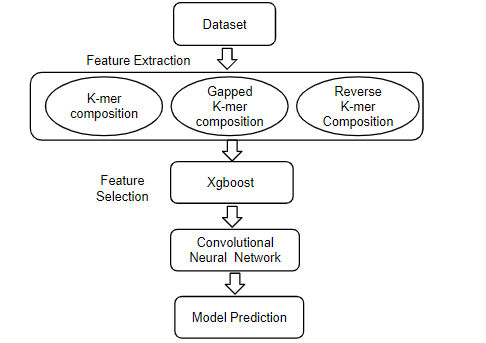
\includegraphics[width=8cm]{images/system.PNG}
    \caption{Model diagram}
    \label{fig:system}
\end{figure}


\subsection{Feature Extraction}
We used three different types of feature extraction techniques.
\subsubsection{ k-mer composition}
 K-mer is the substring of any length k in a sequence.  Counting K-mer is an essential technique in many bioinformatics methods. It also helps on error corrections of sequence reads. We can understand our dataset better using K-mer. Different combinations of data gives us different insights about the dataset. Space capacity is a matter of concern in K-mer. We calculated upto 4 mer here. We extracted 340 features using k-mer composition.
\\

\subsubsection{Gapped k-mer composition}
In order to find a tradeoff between the sparse feature space problem and more sequence composition information, the gapped k-mer has been proposed. Gapped k-mer allows several gaps to exist in k-mers. Therefore, it cannot only significantly reduce the length of the resulting feature vectors, but also takes the evolutionary process into consideration. Experimental results show that this feature is able to obviously improve the performance for enhancer identification. We used gapped k-mer composition till 5 gap and gives 80 features.

The summary of the feature extraction is in the following table \ref{table_1}:
\\


\begin{table}[ht]
\caption{Features summary}
\label{table_1}
\begin{center}
\begin{tabular}{|p{3cm}|p{3cm}|}
\hline
Feature group & number of features\\
\hline
K-mer  & 340\\
\hline
Reverse K-mer  & 340\\
\hline
Gapped k-mer  & 80\\
\hline
\end{tabular}
\end{center}
\end{table}

\subsubsection{Reverse k-mer}
Reverse k-mercomplement is the the reverse complement of DNA sequence. If the sequence is AATCG, then the complement will be CGATT. Reverse complement k-mer often gives hidden and important information from DNA sequence. Reverse composition is just the reverse form of k-mer composition.  Here we used reverse k-mer for extract the features from dataset. Reverse k-mer composition gives 340 features.
\\

\subsection{Feature selection}
We used two types of feature selection methods. We combined all the features found from the feature extraction techniques. 

\subsubsection{Recursive Feature elimination}
Recursive feature elimination (RFE) is a feature selection method that removes the insignificant feature. RFE only chooses features that are applicable for the prediction. This is an iterative process until the desired number of features are achieved. At first it ranked all the dataset according to their importance and then removed them recursively. From different feature subsets, best features with the highest values are selected. 
\\

\subsubsection{Xgboost}
 XGBoost is an implementation of gradient boosted decision trees designed for speed and performance.It is a feature selection technique to reduce unnecessary features.In our implementation, we used Xgboost for more faster. Its really fast when compared to other implementations of gradient boosting.
 
 The summary of the feature selection techniques are in the following table \ref{table_2}
 \begin{table}[ht]
\caption{Feature selection methods}
\label{table_2}
\begin{center}
\begin{tabular}{|p{1cm}|p{1cm}|p{1cm}|p{1cm}|p{1cm}|p{1cm}|}
\hline
Selection model & Acc(\%) & Sn(\%) & Sp(\%) & MCC(\%) & Pc(\%) \\
\hline
Xgboost & 74 & 60 & 86 & 49 & 79\\
\hline
RFE & 69 & 63 & 74 & 37 & 68 \\
\hline

\end{tabular}
\end{center}
\end{table}
\subsection{Classification}
Kernel is one dimension in 1D Convolutional neural network. The model extracts features from sequences data and maps the internal features of the sequence. Convolutional 1D allows to use larger filter sizes. We used 1D CNN on our model after feature selection. Our model gives 77\% accuracy after applying 1D convolutional neural network on 760 features.

\section{Dataset}

The dataset used here is a yeast dataset consisting of DNA sequences of nucleotides with both positive and negative instances. The positive instances are denoted as hotspot and negative are as coldspots. Dataset has 490 DNA segments of hotspot samples(positive) and 591 DNA segments(negative) of coldspot samples. The basic symbols of DNA sequences are A, T, C, G. This dataset represents the set of these sequences. Dataset is slightly imbalanced with less number of positive samples. 

The paper used a yeast DNA sequence dataset. In the paper, CD-HIT is used to reduce the effect of redundancy of similar sequences. After this, the dataset contains a total 1050 samples where 478 are hotspot samples and 572 are coldspot samples. 



\section{RESULTS AND DISCUSSION}



\subsection{Results}
Various models are used to find the result. Different kind of classifiers such as : Support vector classifier (SVC), Gaussian Naive bias (NB), Random forest, adaBoost, Lgistic regression (LR), k neighbours, decision tree and Conv1D are performed.
 
The summary of the classifiers result is in the following table \ref{table_3}
\begin{table}[ht]
\caption{Summary of model result}
\label{table_3}
\begin{center}
    \begin{tabular}{|p{1.4cm}|p{1cm}|p{1cm}|p{1cm}|p{1cm}|p{1cm}|}
\hline
Classifier & Acc(\%) & Sn(\%) & Sp(\%) & MCC(\%) & Pc(\%) \\
\hline
SVC & 76  & 57 & 91 & 52 & 85\\
\hline
GaussianNB & 72 & 60 & 82 & 44 & 74\\
\hline
Random Forest & 75 & 56 & 91 & 51 & 84\\
\hline
AdaBoost & 71 & 59 & 81 & 42 & 73\\
\hline
LR & 67 & 62 & 71 & 33 & 64\\
\hline
K Neighbours & 69 & 56 & 80 & 36 & 70\\
\hline
Decision Tree & 64 & 58 & 69 & 27 & 61\\
\hline
Conv1D  & 77  & 58.58 & 91.49 &  53.98 & 85.55\\
\hline
\end{tabular}
\end{center}
\end{table}

\subsection{Discussion and analysis}
The confusion matrix is used to evaluate accuracy. The confusion matrix gives an output matrix and provides the description of performance of the system. The samples are from two classes: ‘True’ and ‘False,’ and the implementation of the confusion matrix can be done.
There are 4 terms: 1) True positive 2) True negative 3) False positive 4) False negative.
The equations of the evaluation matrix are given bellow: 


\begin{equation}
    Accuracy = \frac{TP+TN}{TP+TN+FP+FN} \newline
    %Recall = \frac{TP}{TP} + FN\\
\end{equation}
\begin{equation}
    Specificity = \frac{TN}{TN+FP} \newline
\end{equation}
\begin{equation}
    Sensitivity = \frac{TP}{TP+FN} \newline
\end{equation}
\begin{equation}
    Precision  = \frac{TP}{TP} +FP \newline
\end{equation}
\begin{equation}
    MCC = \frac{{TP}*{TN} - {FP}*{FN}}{\sqrt{(TP+FP)(TP+FN)(TN+FP)(TN+FN)}} \newline
\end{equation}
\\

Performance comparison of our iRSpot with difffertent existing model is given in the following table \ref{table_4}:
\begin{table}[ht]
\caption{Result comparison}
\label{table_4}
\begin{center}
\begin{tabular}{|p{1.8cm}|p{1cm}|p{1cm}|p{1cm}|p{1cm}|}
\hline
Models & Sn(\%) & Sp(\%) & MCC(\%) & Acc(\%) \\
\hline
RF-DYMHC & 73.01 & 86.56 & 6.49 & 80.40\\
\hline
IDQD & 79.52 & 81.82 & 61.60 & 80.77 \\
\hline
iRSpot-PseDNC & 71.75 & 85.84 & 58.30 & 79.33 \\
\hline
iRSpot-TNCPsecAAC & 76.56 & 70.99 & 47.37 & 73.52\\
\hline
iRSpot-EL & 75.29 & 88.81 & 65.10 & 82.65 \\
\hline
iRSpot-ADOM1575 & 74.88 & 90.04 & 66.13 & 83.14\\
\hline
iRSpot-ADPM & 77.19 & 90.73 & 69.05 & 84.57 \\
\hline
iRSpot-PDI & 71.48 & 92.56 & 66.58 & 83.16 \\
\hline
iRSpot-SF & 84.57 & 75.76 & 69.41 & 84.58 \\
\hline
iRSpot & 58.58 & 91.49 & 53.98 & 77\\ 
\hline

\end{tabular}
\end{center}
\end{table}

\subsubsection{Roc curve}
 The ROC curve is created by plotting the true positive rate (TPR) against the false positive rate (FPR) at various threshold settings. The Roc curve is given in the following figure \ref{fig:roc curve}:
 \begin{figure}[ht]
    \centering
    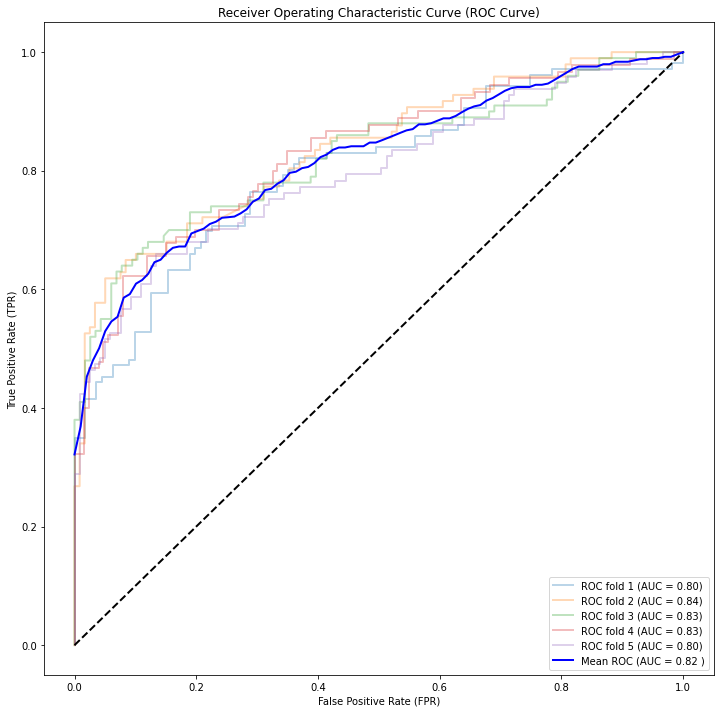
\includegraphics[width=10cm]{images/roc.png}
    \caption{Roc curve}
    \label{fig:roc curve}
\end{figure}

\section{CONCLUSIONS}
We design iRSpot that can predict recombination hotspots. We choose important features using feature elimination techniques. Two different feature slection methods are used to find best result. We use conv1D on total features as conv1D needs a huge number of features for better performance. We wish to improve our model in future. 

%\addtolength{\textheight}{-12cm}  

\section*{ACKNOWLEDGMENT}
The work was done by under the supervision of Rakibul Islam, faculty of United International University. It was a course project of pattern recognition labratory.


%%%%%%%%%%%%%%%%%%%%%%%%%%%%%%%%%%%%%%%%%%%%%%%%%%%%%%%%%%%%%%%%%%%%%%%%%%%%%%%%


\begin{thebibliography}{1}
\bibitem{al2019irspot} Al Maruf, Md Abdullah and Shatabda, Swakkhar, ``iRSpot-SF: Prediction of recombination hotspots by incorporating sequence based features into Chou's Pseudo components,'' 	in Genomics, vol. 111, no. 4, pages: 966--972, Elsevier, 2019. 

\bibitem{yang2018irspot}{2} Yang, Hui and Qiu, Wang-Ren and Liu, Guoqing and Guo, Feng-Biao and Chen, Wei and Chou, Kuo-Chen and Lin, Hao, ``iRSpot-Pse6NC: Identifying recombination spots in Saccharomyces cerevisiae by incorporating hexamer composition into general PseKNC``  in International journal of biological sciences, vol. 14, no. 8, page: 883, Ivyspring International Publisher, 2018

\end{thebibliography}

\end{document}
